\documentclass[12pt,a4paper,titlepage]{jarticle}
\usepackage{layout}
\usepackage[dvips]{graphicx}
\usepackage{float}
\pagestyle{empty}
%\pagestyle{headings}
%\begin{figure}[h]
%\begin{center}
%\includegraphics[width=50mm,height=50mm]{.eps}
%\caption{}
%\end{center}
%\end{figure}
\setlength{\voffset}{-2.5cm}
\setlength{\hoffset}{-30pt}
\setlength{\textwidth}{430pt}
\setlength{\textheight}{680pt}
\begin{document}
%\layout
\title{}
\author{A4SB2121 Yusa Shusaku}
\date{}
%\maketitle

\begin{figure}[h]
\begin{center}
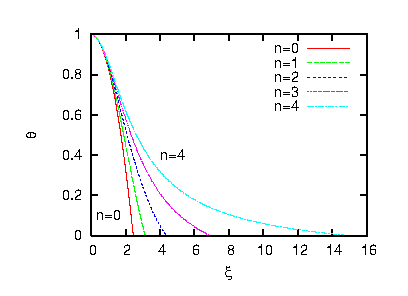
\includegraphics[width=130mm,height=100mm]{Lane_Emden.eps}
\caption{Solution of Lane-Emden Equation}
\end{center}
\end{figure}
The first node����������������Lane-Emden ������


\begin{tabular}{|l|c|}\hline
n & $\xi_1$ \\\hline
0 & 2.4496 \\\hline
1 & 3.1416 \\\hline
2 & 4.3530 \\\hline
3 & 6.8970 \\\hline
4 & 14.972 \\\hline
\end{tabular}
��������������
{\Large$\displaystyle \frac{1}{\xi^2}\frac{d}{d\xi}
\left(\xi^2\frac{d\theta}{d\xi}\right)
 =-\theta^n$ }
\end{document}
